\documentclass[a4paper]{article}
\usepackage[spanish]{babel}
\usepackage[utf8]{inputenc}
\usepackage{float}
\usepackage{graphicx}
%\usepackage[american voltage]{circuitikz}
\usepackage{amsmath}
\usepackage{xcolor}
\usepackage{caption}
\usepackage{subcaption}
\usepackage[bottom]{footmisc}


\begin{document}
	\subsection{Introducción}
	Los amplificadores de instrumentación, también conocidos como \textbf{IN-AMP},  son utilizados para amplificar con alta precisión las señales provenientes de diversas unidades de adquisición de datos que no poseen la amplitud suficiente o estan demasiado contaminadas por ruido externo como para poder ser aprovechadas.
	\subsubsection{Diferencias entre \textbf{IN-AMP} y \textbf{OP AMP}}
	A simple vista un \textbf{IN-AMP} puede ser fácilmente confundido con un \textbf{OP AMP} dado que tiene varios rasgos en común. En primer lugar ambos dispositivos amplifican una señal diferencial, es decir que multiplican por un cierto factor la diferencia de potencial entre sus terminales de entrada. Por otro lado también poseen una elevada impedancia de entrada (del orden de los Megaohms) y una muy baja impedancia de salida de unos pocos ohms.
	No obstante, podemos notar algunas diferencias fundamentales entre ambos. Por ejemplo, para configurar la ganancia a lazo cerrado de un amplificador operacional se debe ajustar mediante resistores de retro-alimentación externos mientras que en un amplificador de instrumentación la ganancia puede venir predefinida por el fabricante o ajustada mediante una única \textbf{resistencia externa} denominada usualmente como \textbf{$R_{gain}$}.
	En caso de que se desee amplificar una señal diferencial el amplificador de instrumentación eliminara cualquier componente de señal común a ambas entradas como puede ser un offset de continua o simplemente ruido. Esta característica es la que hace especiales a los amplificadores de instrumentación ya que permiten reducir de manera significativa el ruido de las señales recibidas.  
	Por el contrario, los amplificadores operacionales tradicionales que no están diseñados para eliminar este tipo señales no deseadas.

	
	\subsection{Características del IN-AMP}
	El circuito a analizar es una variante de los famosos amplificadores de instrumentación que utilizan 3 amplificadores operacionales que se puede observar en la figura debajo.
	%Imagen del amplificador de instrumentación con 3 op-amps
	\begin{figure}[H]
		\centering
		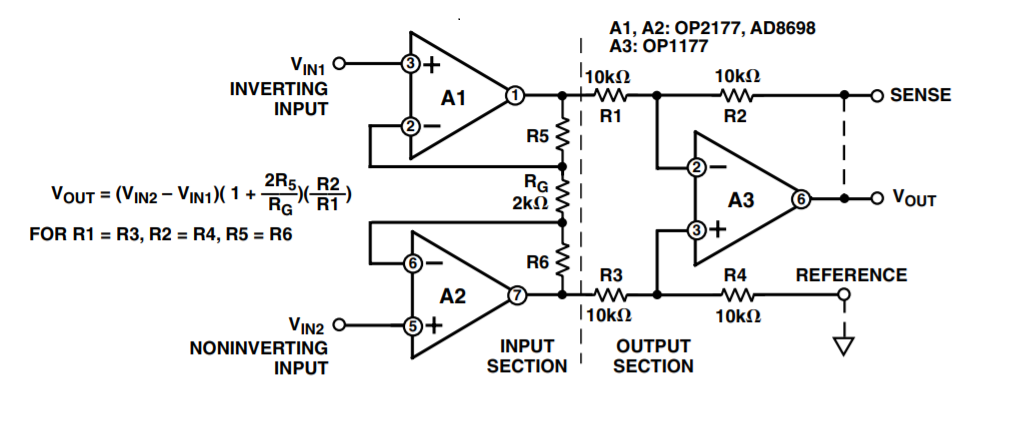
\includegraphics[width=\linewidth]{../ImagenesVarias/inAmp3Opamp}
		%TODO revisar footnote imagen 
		\caption{Clásico amplificador de instrumentación con 3 Opamps}
	\end{figure}
	%\footnote{Imagen extraída de: \textit{A designer's guide to Sinstrumentation amplifiers}
		
	Como se puede apreciar a la izquierda de la línea punteada se han colocado un par de buffers con ganancia. El objetivo de los mismos es de el de aumentar significativamente la impedancia de entrada del in-amp para independizarla lo más posible de la impedancias de las fuentes ya que este pueden ser muy altas o estar desbalanceadas. También ofrece la ventaja de no cargar a la fuente, lo cual es de gran relevancia al trabajar con señales pequeñas. Además le otorga una cierta ganancia a la señal de entrada. Este aspecto del circuito se debe tener en cuenta para evitar la saturación de los op-amps y perder la efectividad del circuito. Analizaremos esta y otras situaciones en secciones posteriores.
	En nuestro caso se trabajara con la versión de 4 amplificadores operacionales.
	
	\begin{figure}[H]
		\centering
		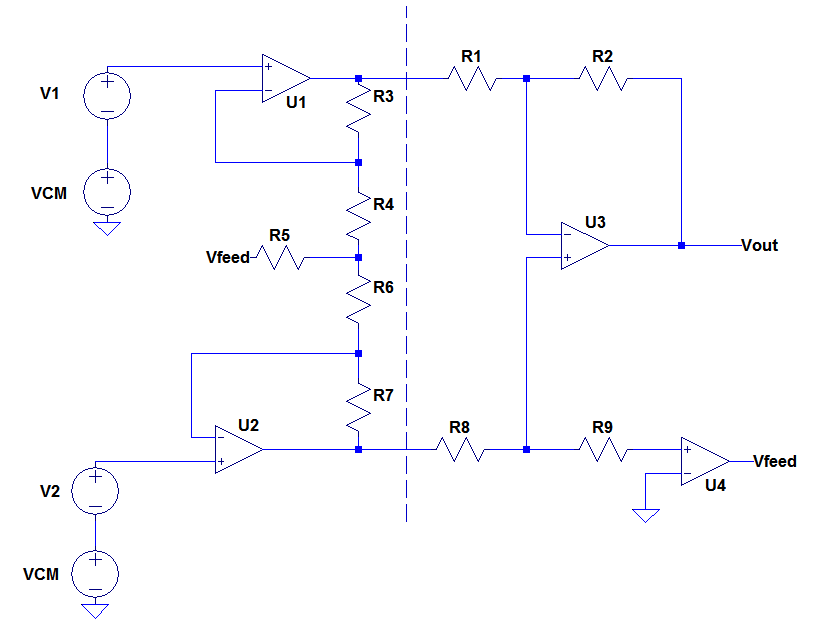
\includegraphics[width=\linewidth]{../ImagenesVarias/inAmpSch.png}
		\caption{Amplificador de instrumentación de 4 op-amps}
	\end{figure}

	Haciendo uso de la herramienta de análisis simbólico \textit{SapWin \footnote{SapWin es una programa de análisis y simulación de circuitos desarrollado por la \textit{Universitá degli studi Firenze}}} obtenemos la siguiente expresión para la ganancia ideal de amplificador de instrumentación:
	\begin{equation}
			V_{out}=\frac{-V_1 R_2 R_4 R_7 - 
			V_1 R_2 R_3 R_7 +
			V_2 R_2 R_3 R_7+
			V_2 R_2 R_3 R_6
		}{R_1 R_4 R_7}
		\label{eqn:idealTrans}
	\end{equation}

	
	Notamos que en la situación ideal tanto las resistencias $R_5$ y $R_9$ no afectan la ganancia del circuito.
	\subsubsection{Relaciones entre los componentes}
	Una de las finalidades del amplificador de instrumentación es la de eliminar aquellas señales que sean comunes a las señales de entrada.
	Por tal motivo comenzaremos por establecer condiciones que nos permitan eliminarlas. 
	Para eso aplicaremos superposición y analizaremos los efectos de $V_{CM}$ sobre la relación anterior.
	
	\begin{figure}[H]
		\centering
		\includegraphics[width=\linewidth]{../ImagenesVarias/inAmpVCM.png}
		\caption{Amplificador de instrumentación de 4 op-amps en modo común}
	\end{figure}
	Obteniendo como transferencia:
	\begin{equation}
		\frac{V_{out}}{V_{CM}}=
		\frac{-R_2 R_4 R_7 - 
			R_2 R_3 R_7 +
			R_2 R_3 R_7+
			R_2 R_3 R_6
		}{R_1 R_4 R_7}
	\end{equation}
		
	Como se quiere que aquellas señales comunes a ambas entrada sean eliminadas pedimos $V_{out}=0$.
	Entonces obtenemos:
		\begin{equation}
		 0=\frac{-V_{CM} R_2 R_4 R_7 - 
				V_{CM} R_2 R_3 R_7 +
				V_{CM} R_2 R_3 R_7+
				V_{CM} R_2 R_3 R_6
			}{R_1 R_4 R_7} 
		\end{equation}
	
	Simplificando
	\begin{equation}
		R_7(R_4+R_3)=R3(R7+R6)
	\end{equation}
	
	\begin{equation}
		R_7R_4+ R_3R_7=R_3R_7+R_3R_6
	\end{equation}
	Cancelando los términos comunes a ambos miembros
	\begin{equation}
		R_7R_4=R_3R_6
	\end{equation}
	Por lo tanto llegamos a:
	\begin{equation}
		\frac{R_4}{R_6}=\frac{R_3}{R_7}  %Relación entre las resistencias de la etapa de amplificación
	\end{equation}

	Aplicando estas relaciones a \eqref{eqn:idealTrans} obtenemos:
	\begin{equation}
		V_{out} = (V_2-V_1)\left[\frac{R_2}{R_1}(1+\frac{R_3}{R_4})\right]
	\end{equation}
En nuestro afán de conseguir una amplificación de 137,32 se realizaron las siguientes consideraciones en busca de conseguir la configuración más simétrica posible.
En primer lugar dadas las limitaciones de las tolerancias de los componentes se decidió implementar un amplificador de instrumentación con una ganancia de 137,5 veces. Sí bien se podría haber intentado calibrar la ganancia del mismo mediante el uso de resistores variables, debemos tener en cuenta que los presets no son ajustables con la suficiente precisión y estos además cuentan con su correspondiente tolerancia. Por otro lado a causa de vibraciones o movimientos bruscos los mismos podrían cambiar su valor forzando al usuario a chequear sus valores previo al uso. 
En segundo lugar se eligieron que las resistencias $R_3$ y  $R_4$ tomasen el mismo valor. Este decisión obligara a que $R_7$ y  $R_6$ también sean iguales. Por lo tanto conseguimos mucha simetría en la primera etapa

\begin{equation}
	V_{out} = (V_2-V_1)\left[2 \frac{R_2}{R_1}\right]
\end{equation}

Luego se eligió $R_2$ del mismo orden de magnitud que $R_1$ de forma tal que el factor de \textbf{2} que apareció previamente sea cancelado y $R_2$ controle por completo la ganancia. Esta $R_2$ fue armada mediante 2 resistores SMD en serie.

\begin{table}[H]
	\centering
	\begin{tabular}{lll}
		Componente  & Valor        	   & Tolerancia \\
		\\
		$R_1$       & 2K$\Omega$   	   & 1\%        \\
		$R_2$       & 130K$\Omega$ 	   & 1\%        \\
		$R_{2'}$  	& 7,5K$\Omega$     & 1\%        \\
		$R_3$ 		& 10K$\Omega$      & 1\%		\\
		$R_4$		& 10K$\Omega$      & 1\%        \\
	    $R_5$		& 10K$\Omega$      & 1\%        \\
	    $R_6$		& 10K$\Omega$      & 1\%        \\
	    $R_7$		& 10K$\Omega$      & 1\%        \\
	    $R_8$		& 2K$\Omega$       & 1\%        \\
 	    $R_9$		& 130K$\Omega$     & 1\%        \\   
		$R_{9'}$	& 7,5K$\Omega$     & 1\%        \\
			\end{tabular}
		\caption{Tabla de valores de componentes del IN-AMP al 1\%}
\end{table}

\begin{figure}[H]
	\centering
	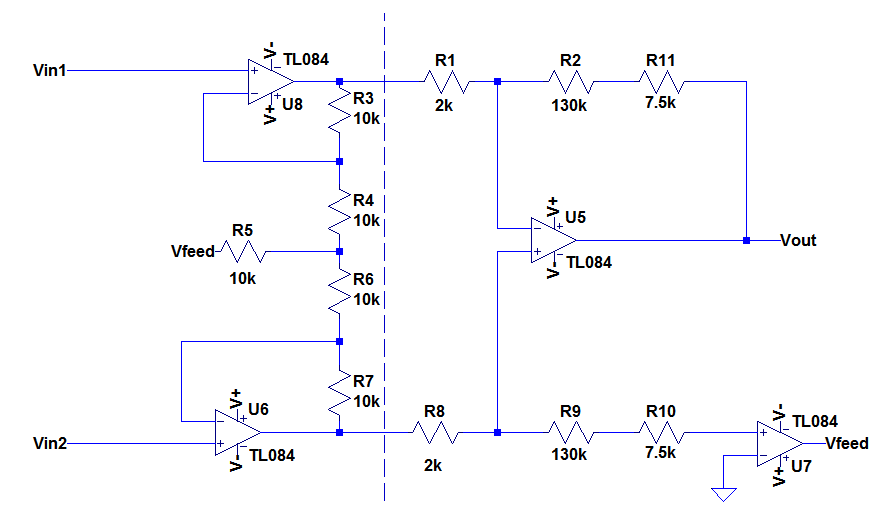
\includegraphics[width=\linewidth]{../ImagenesVarias/IN-AMP-CON-VALORES.png}
	\caption{IN-AMP con los valores elegidos}
\end{figure}

  Cabe destacar que el orden de magnitud de los componentes se baso en que los amplificadores de instrumentación comerciales son fabricados con resistencias en el orden de los K-ohms.
  
  Como fue antes mencionado, el amplificador de instrumentación debe poseer, idealmente, impedancia de entrada infinita. Para poder aproximarnos lo más posible a este ideal se decidió utilizar el amplificador operacional \textbf{TL084} que posee una impedancia de entrada de 1 Tera-Ohm ($10^{12}\Omega$). Otra ventaja de elegir este operacional es que se consiguen en un solo integrado que contiene a los de 4 op-amps dentro de un mismo integrado lo cual disminuye las variaciones por cambios de temperatura dado que se encuentran los 4 bajo las mismas condiciones de operación.
  
\subsection{Efecto de las tolerancias}
Cuando se plantearon los primeros amplificadores diferenciales se utilizaron configuraciones simples como la exhibida debajo, ya se conocía que los resistores $R_1$, $R_2$, $R_3$ y $R_4$ debían estar apropiadamente balanceados con el fin de maximizar el rechazo en modo común. 
\begin{figure}[H]
	\centering
	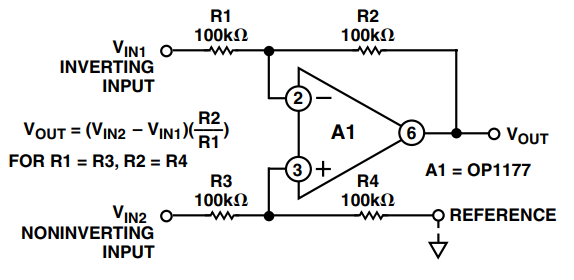
\includegraphics[width=\linewidth]{../ImagenesVarias/AmplificadorDiferencial.PNG}
	\caption{Amplificador diferencial}
\end{figure}  

Sin embargo las tolerancias de los componentes no lo permiten. Es por tal motivo que para alcanzar dicha precisión los fabricantes construyen dichas resistencias, mediante técnicas láser durante el proceso de fabricación del IC con el fin de minimizar esas diferencias.

El modelo más sofisticado y robusto que se implemento presenta mejoras muy notables por sobre su antecesor. No obstante, estas mejoras también traen nuevos desafíos dado que se añaden más componentes resistivos al sistema.

Usando resistencias al 1\% obtenemos la siguiente simulación de Montecarlo para en modo diferencial

\begin{figure}[H]
	\centering
	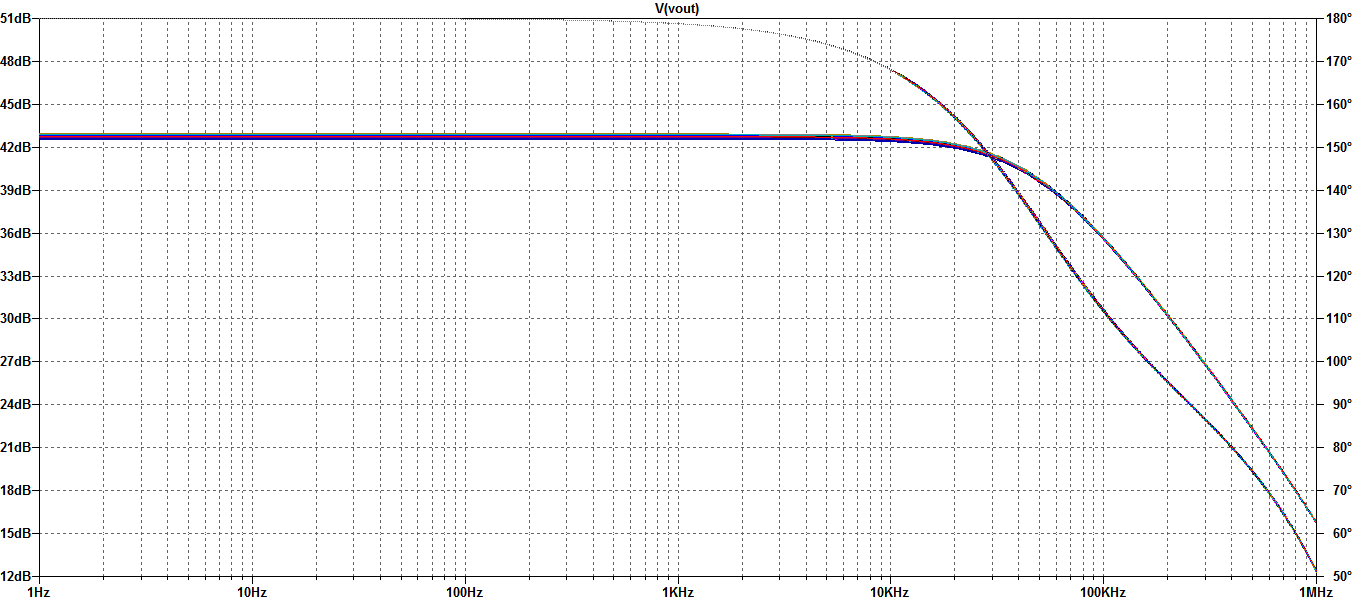
\includegraphics[width=\textwidth]{../ImagenesDeSimulaciones/MonteCarloModoDiferencialGrande.png}
	\caption{Montecarlo en modo diferencial}
\end{figure}  
Como podemos notar, las tolerancias no afectan significativamente su desempeño en modo diferencial.

Sin embargo podemos realizar más observaciones en cuanto a su desempeño en modo comúm
\begin{figure}[H]
	\centering
	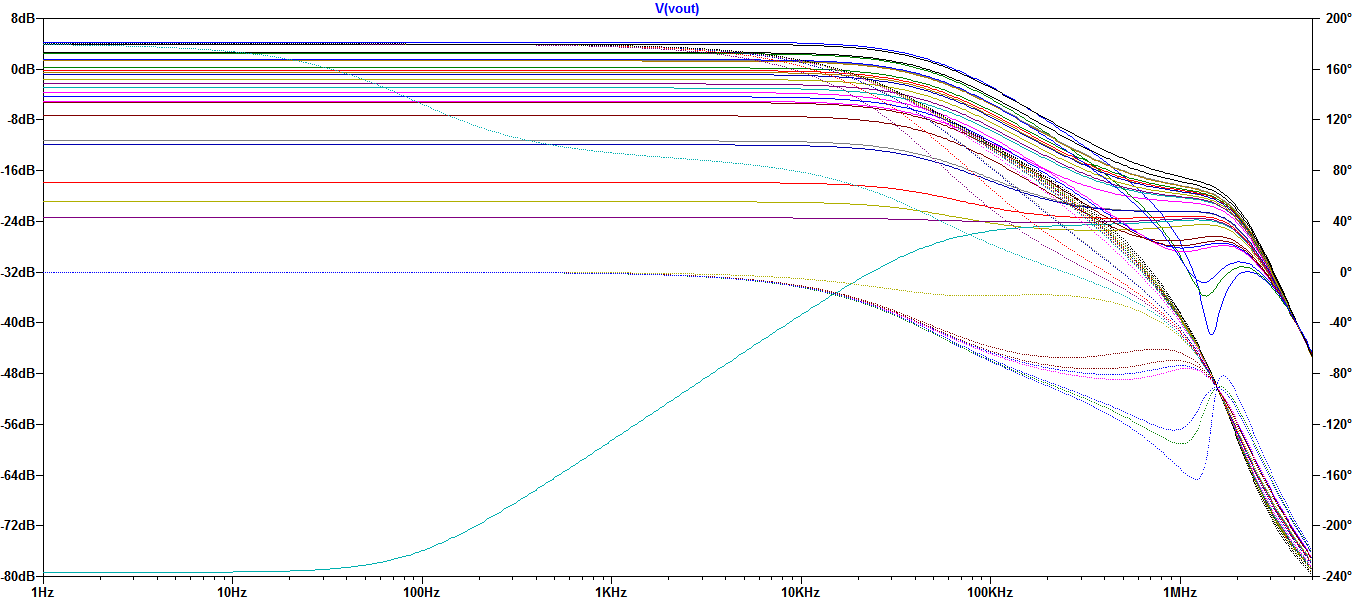
\includegraphics[height=0.3\textheight]{../ImagenesDeSimulaciones/MonteCarloModoComunGrande1V.png}
	\caption{Montecarlo en modo común con 1 Vpp de entrada}
\end{figure} 
Este gráfico de bode pone en evidencia la importancia de que las resistencias poseean la mayor precisión posible.

Si la tensión en modo común se reduce vemos como mejora el rechazo en modo común.
\begin{figure}[H]
	\centering
	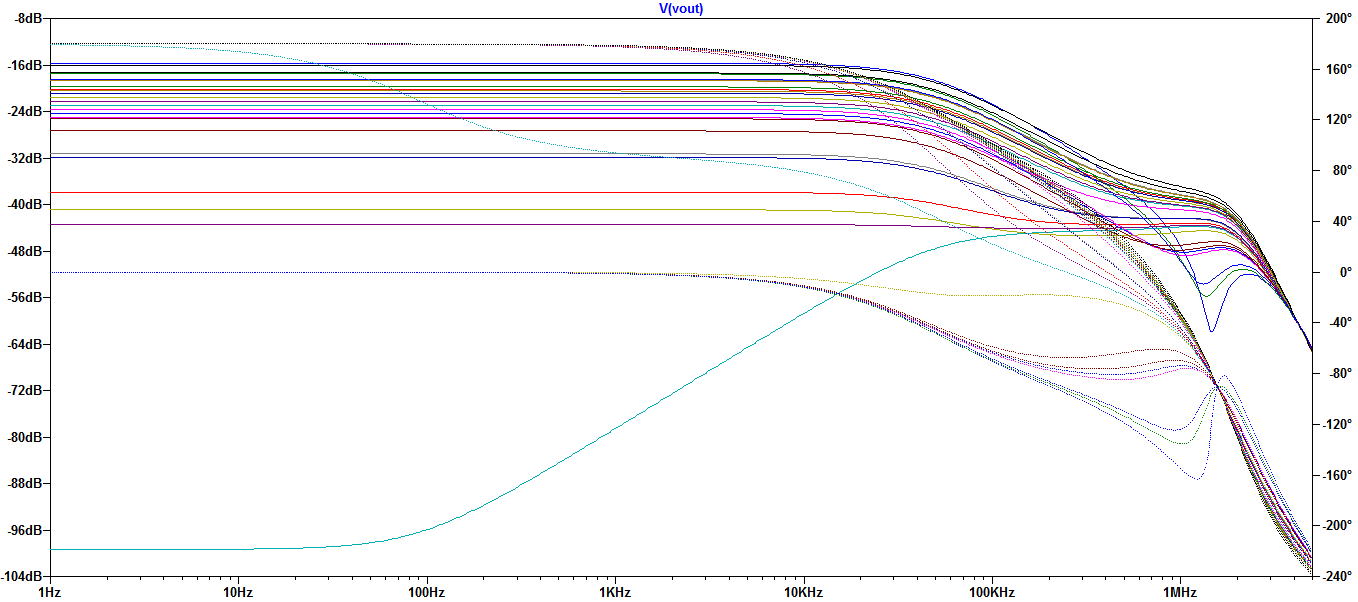
\includegraphics[height=0.3\textheight]{../ImagenesDeSimulaciones/MonteCarloModoComunGrande100mv.png}
	\caption{Montecarlo en modo común con 100 mv de entrada}
\end{figure} 

También se intento ver los alcances de rechazo común frente a una continua
\begin{figure}[H]
	\centering
	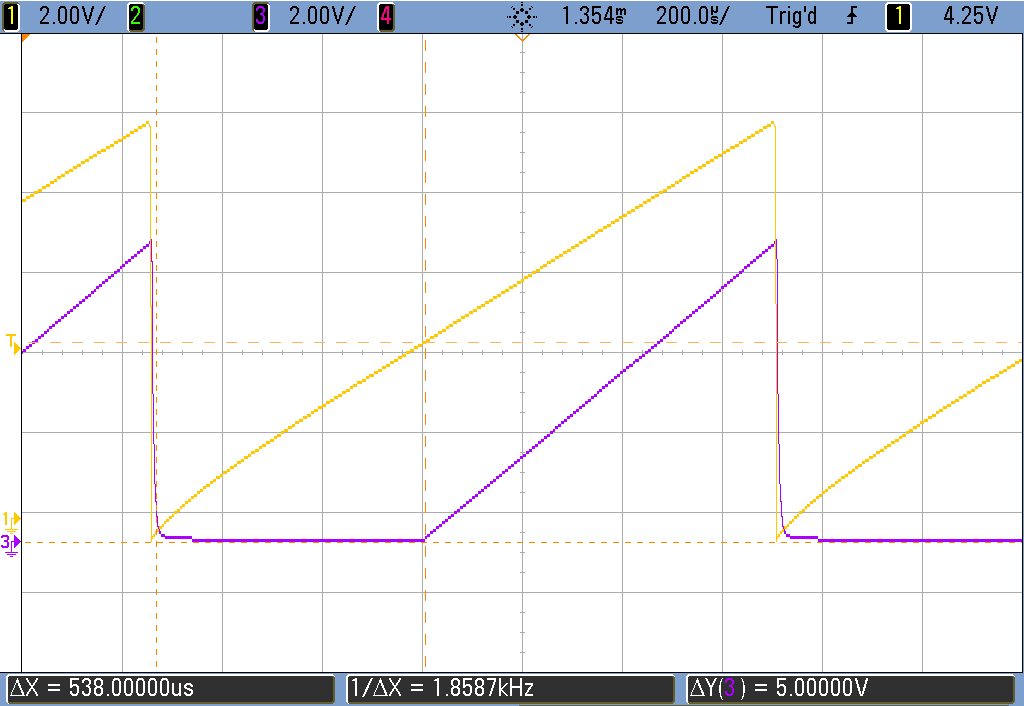
\includegraphics[height=0.3\textheight]{../ImagenesDeOsciloscopio/ModoComunContinua.png}
	\caption{Rampa de 0 a 20V}
\end{figure} 

Vemos como el circuito es capaz de soportar hasta unos 5V de continua (como indica el cursor) antes de salir de su zona de operación.

\subsection{Respuesta en frecuencia}
Los amplificadores de instrumentación obtienen su mejor rendimiento en la rango de las frecuencias medias a bajas. Esta configuración exhibe un comportamiento del tipo pasabajos lo que provoca que no se obtenga la ganancia esperada a frecuencias elevadas.
\begin{figure}[H]
	\centering
	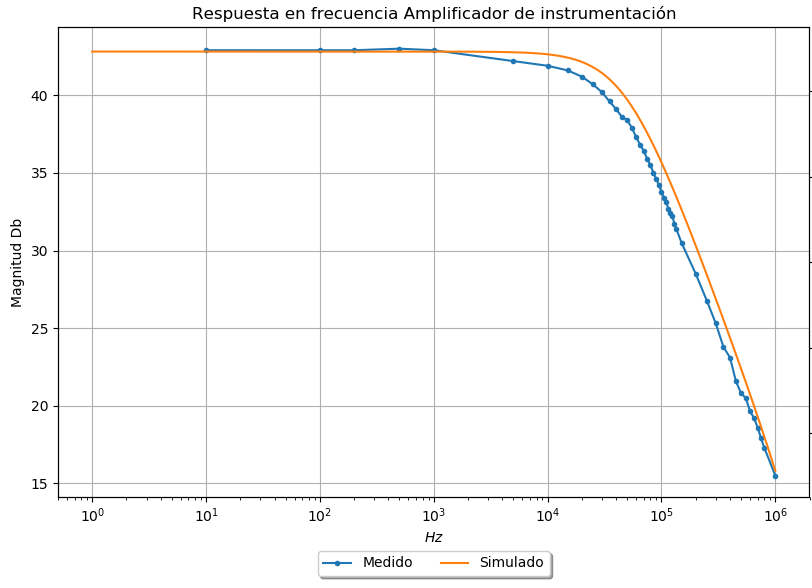
\includegraphics[height=0.3\textheight]{../ImagenesVarias/BODE_MAG.PNG}
	\caption{Bode de Magnitud}
\end{figure}


  
  
  
  
  
  
  
  
  
  
  
  
  
  
  
  
  
\subsection{Generación de señales con puente de Wheatstone}
Se diseño un puente de WheatStone para la generación de señales compuestas.
\begin{figure}[H]
	\centering
	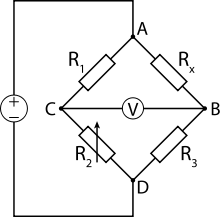
\includegraphics[height=0.25\textheight]{../ImagenesVarias/wheatstone.png}
	\caption{Puente de WheatStone}
\end{figure}

Este método emula a un sensor que utilice un sistema tipo puente con un resistor variable que puede llegar a cambiar de valor según la temperatura, presión u alguna otra que ocasiona que su valor cambie.

\begin{figure}[H]
	\centering
	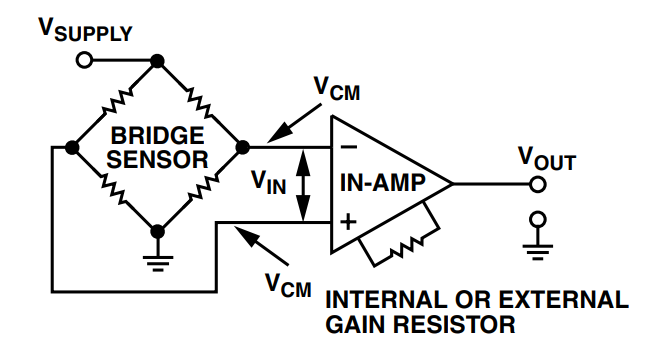
\includegraphics[height=0.3\textheight]{../ImagenesVarias/wheatstoneInAmp.png}
	\caption{IN-AMP con puente de WheatStone Acoplado}
\end{figure}

La tensión suministrada en la parte superior del puente permite que las variaciones de resistencia se traduzcan en una señal eléctrica.
Sin embargo es necesario poseer una cierta referencia para poder determinar si de hecho ocurrió un cambio. Es por es que el amplificador de instrumentación se vale del puente y de sus 2 bornes de salida para llevar acabo esta detección. La rama del puente que cuenta con sus resistores fijos proporcionara la tensión de referencia.
A la entrada del amplificador de instrumentación se le proporcionaran 2 señales. En primer tendremos la señal de referencia y por el otro la señal portadora de la perturbación.
Debemos notar que dado el diseño del amplificador de instrumentación de no haber diferencias entre las dos señales entonces en el caso ideal se debería observar una salida nula. 

Para el armado del puente se eligieron resistores con tolerancias del 1\% para mantener el puente lo más balanceado posible y maximizar el rechazo en modo común.
\begin{table}[H]
	\centering
	\begin{tabular}{lll}
		Componente  		& Valor        	& Tolerancia \\
		\\
		$R_1$       		& 10K$\Omega$   & 1\%        \\
		$R_2$       		& 10K$\Omega$ 	& 1\%        \\
		$R_{2'}$ Preset      & 1K$\Omega$ 	& 10\%        \\
		$R_3$  				& 10K$\Omega$   & 1\%        \\
		$R_4$ 				& 10K$\Omega$   & 1\%		\\
	\end{tabular}
	\caption{Tabla de valores de componentes del puente de WheatStone al 1\%}
\end{table}

El preset nos permite generar de manera artificial "la perturbación" sobre la señal.

\begin{figure}[H]
	\centering
	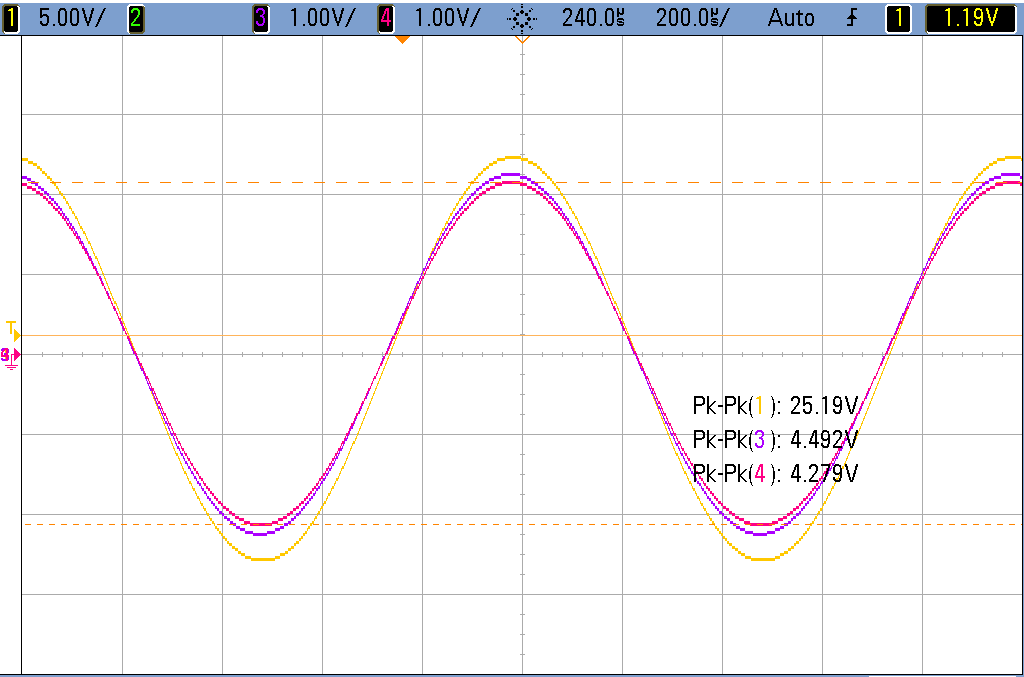
\includegraphics[height=0.3\textheight]{../ImagenesDeOsciloscopio/WheatStone1tierra1c1R.png}
	\caption{Amplificación de diferencias con puente de WheatStone}
\end{figure}
Notese la escala de las señales.
\subsubsection{Análisis de Tolerancias en el puente de WheatStone}


\subsubsection{Señales con y sin referencia a tierra}
El amplificador de instrumentación es destacado por su capacidad de suprimir el ruido presente en una señal diferencial. La clave de este dispositivo esta en que la contaminación es la misma para ambos canales.
Al compartir la referencia entre el generador de la señal y el \textbf{IN-AMP} ambos estan sujetos a la misma contaminación externa que se genera respecto de su potencial de referencia (GND). Por el otro lado si estos dos no comparten referencia entonces dichas contaminaciones se generaran contra tensiones de referencia diferentes lo cual provocara que se adicione al ruido en las terminales del amplificador de instrumentación  



 	
\begin{thebibliography}{9}
	
	\bibitem{Franco} 
	SERGIO, F. (2002). Design with operational amplifiers and analog integrated circuits. New York [etc.]: McGraw-Hill, pp.73-91.	
	
	\bibitem{Coughlin} 
	R. Coughlin and F. Driscoll, Circuitos integrados lineales y amplificadores operacionales. México: Prentice-Hall Hispanoamericana, 1998.
	
	\bibitem{dguideinamp}
	C. Kitchin and L. Counts, A designer's guide to instrumentation amplifiers. Norwood, Mass.: Analog Devices, 2006.
	
	\bibitem{an244}
	Jeffrey R. Riskin, A User's guide to IC instrumentation amplifiers. Norwood, Mass.: Analog Devices.
	
\end{thebibliography}

\end{document}